\chapter{Apache Kafka nel settore dell’Integrazione Aziendale}

% \section{L’evoluzione delle architetture di integrazione}
%
% % Introduzione al motivo aziendale per cui è nato questo percorso di stage: la propensione odierna alle architetture a microservizi, la gestione di grandi flussi di dati in modo efficiente ed eff1icace, una richiesta di un sistema innovativo da parte della clientela.3
% L'evoluzione del settore dell'\textit{Enterprise Application Integration} verso soluzioni sempre più distribuite e con un flusso di dati in continuo aumento ha sviluppato nei clienti (e di conseguenza nell'azienda) un interesse verso il prodotto Apache Kafka.
% Il software ha dimostrato negli anni recenti un notevole successo in diversi campi; l'azienda ha interesse nel testare le capacità di Kafka nel soddisfare le esigenze dell'integrazione aziendale.
%
% \bigskip
% \begin{figure}[h]
%   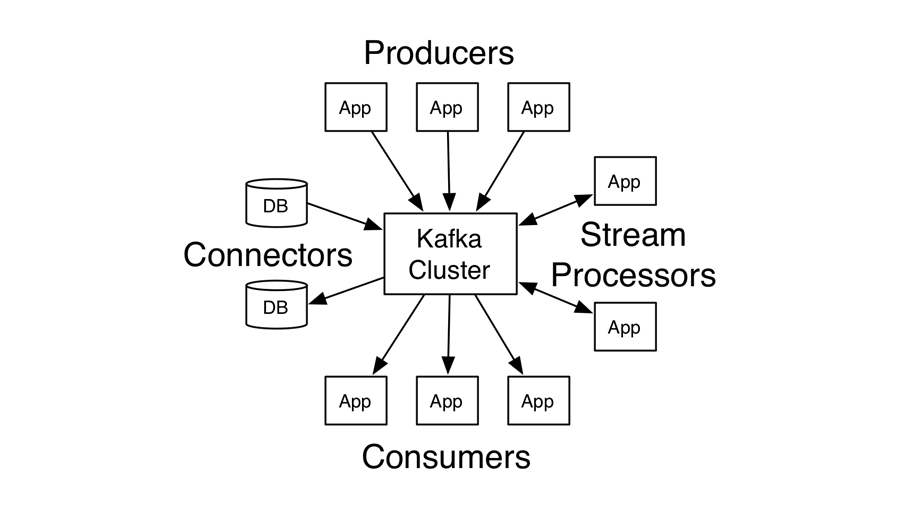
\includegraphics[width=\textwidth]{images/kafka.png}\\
%   \caption{Illustrazione di un sistema a servizi con Apache Kafka}
%   \captionsetup{aboveskip=2pt,font=it}
%   \caption*{Fonte: https://kafka.apache.org/20/documentation.html}
% \end{figure}
%
% Kafka è una piattaforma di \textit{event streaming}, un sistema moderno e distribuito basato sugli eventi anzichè su di una soluzione più classica come può essere quella del \textit{request/response}.
% L'adozione del \textit{software} nell'ambito dell'EAI è in crescita dato le dimostrate qualità nel gestire grandi moli di dati: la sua performance, sicurezza e scalabilità sono i punti che hanno portato il software al suo attuale successo.
%
% % \bigskip\noindent
% % Esposizioni delle ragioni personali che hanno portato alla scelta di tale percorso.


\section{Apache Kafka come Middleware}

L'interesse aziendale nel \textit{software} risiede nell'utilizzo di Kafka come un  \textit{Middleware}, ovvero di un sistema che consenta la comunicazione tra differenti servizi con un rapido flusso di dati fra di essi.
L'azienda ha avviato un percorso per testare le capacità di Kafka rispetto agli attuali strumenti utilizzati nel settore, per valutare i vantaggi e svantaggi che l'adozione di tale software può fornire al cliente.

\bigskip\noindent
Sono numerosi i vantaggi che Kafka può portare nel settore, fra cui:
\begin{itemize}
  \item gestione performante di un enorme flusso di dati;
  \item scalabilità;
  \item sicurezza riguardo la persistenza dei dati;
  \item semplice integrazione e affiancamento a sistemi già esistenti;
  \item l'essere una piattaforma \textit{open source};
  \item processazione dei dati integrata.
\end{itemize}


%
% \bigskip\noindent
% Come Kafka possa risolvere i problemi e le necessità viste qui sopra.

\section{Il percorso di Stage}

% Descrizione di come il percorso di \textit{stage} si inserisce nella visione più ampia riportata qui sopra.
%
% \bigskip\noindent
% Elenco degli obiettivi del percorso:
% \begin{itemize}
%   \item formazione riguardo Kafka e l’ambito dell’integrazione;
%   \item verificare le capacità di Kafka nell’ambito EAI;
%   \item sperimentare l’utilizzo di Kafka come \textit{Middleware} tramite una simulazione di un caso d’uso reale a servizi indipendenti.
% \end{itemize}
%
% \noindent
% Breve esposizione dei motivi che mi hanno portato a scegliere questo percorso

Il percorso di \textit{stage} offerto dall'azienda si inserisce all'interno della strategia aziendale più ampia descritta qui sopra.
La proposta riguarda infatti la sperimentazione di Apache Kafka in un caso d'uso simulato nell'ambito delle telecomunicazioni, ispirato ad un caso d'uso reale.

L'obiettivo principale dello \textit{stage} è lo sviluppo di un'architettura basata su Kafka con conseguente reingegnerizzazione dei flussi di integrazioni preesistenti; lo studente ha il compito di osservare, testare e verificare che il \textit{software} possa svolgere alcuni compiti inerenti all'area dell'EAI, analizzando alcuni casi d'uso presenti in un \textit{Middleware} aziendale in ambito \textit{telco}.

\bigskip\noindent
Il percorso proposto prevede le seguenti attività e obiettivi:
\begin{itemize}
  \item formazione riguardo la piattaforma di \textit{event streaming} Kafka e l'ambito dell'integrazione aziendale;
  \item verifica delle capacità di Kafka nell'EAI;
  \item sperimentazione e sviluppo di un \textit{Middleware} basato su Kafka tramite una simulazione di un caso d'uso reale a servizi indipendenti.
\end{itemize}

La ragione principale che mi ha portato a scegliere questo percorso di \textit{stage} è l'interesse verso Apache Kafka, la cui formazione ritengo possa arricchire fortemente le mie capacità professionali.
L'utilizzo della piattaforma di \textit{event streaming} è sempre più in crescita, come l'evoluzione verso sistemi sempre più distribuiti e a microservizi.
Altri fattori fondamentali alla scelta del percorso sono stati la famigliarità con l'azienda, il loro metodo di lavoro e la libertà di sviluppo: ho valutato positivamente la possibilità di elaborare personalmente un'architettura del caso d'uso con una visione ad alto livello anzichè il semplice sviluppo di un software predeterminato.
